%!TeX program = xelatex

%
% O MODELO DESTE DOCUMENTO É abntex2-modelo-trabalho-academico.tex
% HÁ MAIS SEÇÕES NO MODELO DO QUE NESTE ARQUIVO AQUI.
% É PARA CONSTRUIR AOS POUCOS.
%
%
\documentclass[
% -- opções da classe memoir --
12pt,				% tamanho da fonte
openright,			% capítulos começam em pág ímpar (insere página vazia caso preciso)
%twoside,			% para impressão em recto e verso. Oposto a oneside
oneside,			% VAMOS EVITAR AS PÁGINAS EM BRANCO ENTRE OS CAPÍTULOS?
a4paper,			% tamanho do papel. 
% -- opções da classe abntex2 --
chapter=TITLE,		% títulos de capítulos convertidos em letras maiúsculas
%section=TITLE,		% títulos de seções convertidos em letras maiúsculas
%subsection=TITLE,	% títulos de subseções convertidos em letras maiúsculas
%subsubsection=TITLE,% títulos de subsubseções convertidos em letras maiúsculas
% -- opções do pacote babel --
english,			% idioma adicional para hifenização
brazil				% o último idioma é o principal do documento
]{abntex2}

\usepackage{_estilos}
\usepackage{_listings}


% ====================================================================================================================================
% ---
% Informações de dados para CAPA e FOLHA DE ROSTO
% ---
\titulo{Abordagens para mitigação de riscos de segurança da informação em navegadores: uma proposta baseada em JavaScript e HTML}
\autor{Humberto Borgas Bulhões}
\local{São Paulo}
\data{2018}
\mes{Janeiro}

\orientador{Prof. Dr. Marcelo Novaes de Rezende}
\orientadorafiliacao{IPT -- Instituto de Pesquisas Tecnológicas do Est. de SP}
\membroum{Prof. Dr. Alexandre José Barbieri de Sousa}
\membroumAfiliacao{Mestrado em Engenharia de Computação}
\membrodois{Prof. Dr. Plínio Roberto Souza Vilela}
\membrodoisAfiliacao{Universidade Estadual de Campinas -- UNICAMP}
%\suplente{Prof. Dr. Francisco Isidro Massetto}
%\suplenteAfiliacao{Universidade Federal do ABC -- UFabc}

\instituicao{\mbox{Instituto} de Pesquisas Tecnológicas do \mbox{Estado} de São Paulo}
\tipotrabalho{Dissertação de Mestrado}
\curso{Engenharia da Computação: Engenharia de Software}
\concentracao{Área de Concentração: Engenharia de \mbox{Software}}
\tipotrabalho{Dissertação de Mestrado}
\palavraschave{Segurança da informação, vazamento de dados, HTML, Javascript, DOM.}
\keyword{Information security, information leak, HTML, Javascript, DOM.}
% O preambulo deve conter o tipo do trabalho, o objetivo, 
% o nome da instituição e a área de concentração 
\preambulo{Exame de Qualificação apresentado ao
	Instituto de Pesquisas Tecnológicas do
	Estado de São Paulo – IPT, como parte
	dos requisitos para a obtenção do título
	de mestre em Engenharia de
	Computação.}
% ---

% ====================================================================================================================================
% ---
% compila o indice
% ---
%\makeindex
% ---

% ====================================================================================================================================
% ----
% Início do documento
% ----
\begin{document}
	
	\chapterstyle{iptabntex2}			% Estilo de capitulo adotado pelo IPT
	
	% Retira espaço extra obsoleto entre as frases.
	\frenchspacing
	
	% ----------------------------------------------------------
	% ELEMENTOS PRÉ-TEXTUAIS
	% ----------------------------------------------------------
	\pretextual
	%!TEX root = Projeto.tex
\imprimircapa
\imprimirfolhadeaprovacao
\imprimirfolhaderosto

% ---
% Inserir a ficha bibliografica
% ---

% Isto é um exemplo de Ficha Catalográfica, ou ``Dados internacionais de
% catalogação-na-publicação''. Você pode utilizar este modelo como referência.
% Porém, provavelmente a biblioteca da sua universidade lhe fornecerá um PDF
% com a ficha catalográfica definitiva após a defesa do trabalho. Quando estiver
% com o documento, salve-o como PDF no diretório do seu projeto e substitua todo
% o conteúdo de implementação deste arquivo pelo comando abaixo:
%
% \begin{fichacatalografica}
%     \includepdf{fig_ficha_catalografica.pdf}
% \end{fichacatalografica}
\begin{fichacatalografica}
	\vspace*{\fill}					% Posição vertical
	\hrule							% Linha horizontal
	\begin{center}					% Minipage Centralizado
	\begin{minipage}[c]{12.5cm}		% Largura

	\imprimirautor

	\hspace{0.5cm} \imprimirtitulo  / \imprimirautor. --
	\imprimirlocal, \imprimirdata-

	\hspace{0.5cm} \pageref{LastPage} p. : il. (algumas color.) ; 30 cm.\\

	\hspace{0.5cm} \imprimirorientadorRotulo~\imprimirorientador\\

	\hspace{0.5cm}
	\parbox[t]{\textwidth}{\imprimirtipotrabalho~--~\imprimirinstituicao,
	\imprimirdata.}\\

	\hspace{0.5cm}
%		1. Palavra-chave1.
%		2. Palavra-chave2.
%		I. Orientador.
%		II. Universidade xxx.
%		III. Faculdade de xxx.
%		IV. Título\\

	\hspace{8.75cm} CDU 02:141:005.7\\

	\end{minipage}
	\end{center}
	\hrule
\end{fichacatalografica}
% ---



% ---
% Dedicatória
% ---
%\begin{dedicatoria}
%\vspace*{\fill}
%\OnehalfSpacing
%%\centering
%%\noindent
%Dedico este trabalho...
%
%
%\vspace*{\fill}
%\end{dedicatoria}
% ---

% ---
% Agradecimentos
% ---
%\begin{agradecimentos}
%\vspace*{\fill}
%\OnehalfSpacing
%Gostaria de agradecer...
%
%
%\vspace*{\fill}
%\end{agradecimentos}
% ---

% ---
% Epígrafe
% ---
%\begin{epigrafe}
%    \vspace*{\fill}
%	\begin{flushright}
%		\textit{``Não vos amoldeis às estruturas deste mundo, \\
%		mas transformai-vos pela renovação da mente, \\
%		a fim de distinguir qual é a vontade de Deus: \\
%		o que é bom, o que Lhe é agradável, o que é perfeito.\\
%		(Bíblia Sagrada, Romanos 12, 2)}
%	\end{flushright}
%\end{epigrafe}
% ---


%!TEX root = Projeto.tex
\newpage
\begin{resumo}
\normalsize

Impulsionados por recursos avançados de HTML e Javascript, os programas navegadores da web tornaram-se plataformas de desenvolvimento e publicação de aplicativos. O aumento em escopo de funcionalidade dos navegadores, porém, vem acompanhado de vulnerabilidades de segurança da informação que podem expor dados do usuário. Muitas dessas vulnerabilidades se manifestam de formas sutis, mantendo-se fora do alcance das políticas de segurança padronizadas e adotadas pela indústria, e afetando a confidencialidade da informação que trafega pelo navegador. Para neutralizar esse problema diversas iniciativas experimentais têm sido propostas, sem que tenham encontrado, até o momento, adoção em massa. Ao mesmo tempo, novos recursos de programação têm sido incorporados aos navegadores, e alguns deles, quando utilizados em conjunto, levantam a possibilidade de implementação do encapsulamento da informação, tornando-a invisível a agentes não autorizados. O objetivo deste trabalho é propor um método que, fundamentado em capacidades de programação padronizadas e difundidas, implemente o encapsulamento da informação em HTML e Javascript, o que poderia tornar realidade alguns dos requisitos de segurança que apenas abordagens experimentais têm conseguido assegurar. Para tanto, este trabalho apresentará uma especificação desse método, uma implementação modelo e uma avaliação da eficácia do método em relação a determinados casos de teste que evidenciam problemas de confidencialidade da informação.

\vspace{\onelineskip}

\noindent
\textbf{Palavras-chave:} \imprimirpalavraschave
\end{resumo}

% resumo em inglês
%\begin{resumo}[Abstract]
%%\begin{otherlanguage*}{english}
%Resumo da dissertação em inglês.
%
%
%\vspace{\onelineskip}
%
%\noindent
%\textbf{Keywords:} \imprimirkeyword   
%%\end{otherlanguage*}
%\end{resumo}

% ---
% inserir lista de ilustrações
% ---
{\SingleSpacing
\pdfbookmark[0]{\listfigurename}{lof}
\listoffigures*
\cleardoublepage
}
% ---

% ---
% inserir lista de trechos de código fonte
% ---
{\SingleSpacing
	\pdfbookmark[0]{\lstlistlistingname}{lol}
	\lstlistoflistings
	\cleardoublepage
}
% ---

% ---
% inserir lista de quadros
% ---
%\pdfbookmark[0]{\listofquadrosname}{loq}
%\listofquadros*
%\cleardoublepage
% ---

% ---
% inserir lista de tabelas
% ---
%{\SingleSpacing
%\pdfbookmark[0]{\listtablename}{lot}
%\listoftables*
%\cleardoublepage
%}
% ---

% ---
% inserir lista de abreviaturas e siglas
% ---
%
\begin{siglas}
  \item[CORS] Cross-Origin Resource Sharing
  \item[CSRF] Cross-Site Request Forgery
  \item[DAC] Discretionary Access Control
  \item[DOM] Document Object Model
  \item[IFC] Information Flow Control
  \item[JSON] JavaScript Object Notation
  \item[MAC] Mandatory Access Control
  \item[SOP] Same Origin Policy
  \item[XSS] Cross-Site Scripting
\end{siglas}

% ---

% ---
% inserir lista de símbolos
% ---
%\begin{simbolos}
%  \item[$ \Gamma $] Letra grega Gama
%  \item[$ \Lambda $] Lambda
%  \item[$ \zeta $] Letra grega minúscula zeta
%  \item[$ \in $] Pertence
%\end{simbolos}
% ---

% ---
% inserir o sumario
% ---
{\SingleSpacing
	\cleardoublepage
	\pdfbookmark[0]{\contentsname}{toc}
	\tableofcontents*
	\cleardoublepage
}
% ---
	
	
	% ----------------------------------------------------------
	% ELEMENTOS TEXTUAIS
	% ----------------------------------------------------------
	\textual
	\OnehalfSpacing
	
	%!TEX root = Projeto.tex
\chapter{Introdução}

 %!TEX root = Projeto.tex
\section{Motivação}

%ESTÁ MUITO CONFUSO. MELHOR COMEÇAR DIRETO AO PONTO COMO O DEIAN. DEIXAR EVIDENTE A DISTÂNCIA ENTRE O ESTADO DA ARTE E O ESTADO DAS FERRAMENTAS, E POR QUE ISSO COMPLICA A VIDA DE DESENVOLVEDORES E USUÁRIOS. ESCREVER PENSANDO QUE O OBJETIVO DO TRABALHO É ""AVALIAR"" UMA ALTERNATIVA AO ESTADO DA ARTE, SEM EFETIVAMENTE DIZÊ-LO AQUI.

É difícil desenvolver aplicações seguras para a web. Mesmo sob a defesa de \textit{firewalls}, protocolos de segurança, software antivírus e atualizações periódicas dos navegadores, as informações dos usuários permanecem fundamentalmente expostas ao acesso indevido por \textit{scripts} mal-intencionados ou mal-escritos. Essa condição se expressa de forma crítica por meio do chamado conteúdo ativo, recurso do navegador que viabiliza a existência de aplicações interativas nas linguagens HTML e Javascript. Criar um \textit{script} com a intenção de ler o conteúdo potencialmente sigiloso de uma página da web e revelá-lo a terceiros não-autorizados é uma tarefa que exige pouca habilidade e que pode passar despercebida pelo aparato de segurança disponível.

Exemplos de manipulação maliciosa de scripts incluem sequestro de redes de distribuição de conteúdo (CDN, \textit{content distribution network}) \cite{Dorfman2013}, injeção de scripts por extensões, por vírus ou por redirecionamento \cite{Kinlan2015}, e ainda a inclusão de código não verificado pelo publicador \cite{Vanunu2016}. Tais tipos de ataques não tiram proveito de defeitos dos navegadores; ao invés disso, funcionam de acordo com os mecanismos de segurança da informação padronizados pela indústria. Isto ocorre porque parte da tecnologia que dá suporte ao conteúdo ativo é fundamentalmente limitada no nível de segurança da informação que pode oferecer, especialmente quando é considerado o rico ambiente de execução proporcionado pelo software navegador. Nele, a confidencialidade da informação é vulnerável a agentes maliciosos que operam em dois âmbitos:

\begin{alineas}
	\item Componentes de \textit{script} incorporados às páginas da web são executados com os mesmos privilégios e mesmo nível de acesso à página como um todo \cite[p. 2-3]{DeRyck2012}, sejam eles benignos ou não. O navegador oferece diretivas de segurança limitadas para conter o vazamento de informação entre componentes, uma vez que não há um meio de especificar relações de confiança entre eles \cite{Jang2010}.
	\item \textit{Plugins} e extensões do navegador têm nível de acesso mais elevado aos recursos de sistema do que aquele definido para componentes de páginas da web, permitindo que \textit{plugins} tomem controle de funcionalidades como gerenciamento de conexões de rede, eventos de navegação e o DOM. Ainda que dependam da permissão explícita do usuário no momento de sua instalação, os \textit{plugins} e extensões podem se comportar como agentes de vazamento de informação de forma sutil e não necessariamente proposital \cite{Heule2015_Most_Dangerous_Code}.
\end{alineas}

Na raiz das vulnerabilidades está a forma inconsistente e parcial com que a linguagem Javascript e as APIs do navegador tratam o isolamento entre \textit{scripts} e dados. A caracterização e a solução desse problema fazem parte de um campo de pesquisas ativo \cite{Stefan2014}, \cite{Hedin2014}, \cite{Bichhawat2014}, \cite{Magazinius2014} e em busca por padronização \cite{W3C:WebAppSec}, mas que ainda não resultou em práticas, ferramentas e protocolos de amplo alcance pois dependem da adoção de políticas de segurança experimentais \cite{Hedin2014}, \cite{Bichhawat2014} e potencialmente degradantes de desempenho \cite[p. 14]{Stefan2014} por parte dos desenvolvedores de navegadores.

No campo das tecnologias experimentais estão as estratégias baseadas no controle do fluxo da informação (IFC, \textit{information flow control}). IFC, inicialmente descrito por \cite{Denning1976}, estabelece que cada espaço de armazenamento em um programa -- arquivos, segmentos de memória, conexões de rede ou variáveis, por exemplo -- seja rotulado por uma classe de segurança. Em função disso, o trânsito de informação entre espaços de armazenamento deve ser monitorado e, eventualmente, interrompido quando os rótulos da origem e do destino da informação não forem compatíveis. IFC é um mecanismo inexistente nas implementações da linguagem Javascript dos navegadores da web; implementá-lo em uma linguagem dinâmica como Javascript significa introduzir uma checagem de rótulos a cada leitura e escrita em objetos mutáveis \cite[p.3]{Heule2015_IFC_Inside}, acarretando perdas significativas na velocidade da execução de \textit{scripts}.

Os desenvolvedores de aplicações em conteúdo ativo, por sua vez, têm limitadas opções para a publicação de \textit{sites} e páginas web seguras. Ainda que sigam as práticas recomendadas para a neutralização dos ataques mais comuns à segurança da informação \cite{W3C:CORS}, \cite{W3C:SOP}, \cite{W3C:CSP}, o conteúdo das páginas da web permanece acessível aos \textit{scripts} incorporados e às extensões do navegador.





%!TEX root = Projeto.tex
\section{Objetivo}

%A MOTIVAÇÃO DEVE TER ESCLARECIDO QUE EXISTEM PROBLEMAS DE INFOSEC DIFÍCEIS DE SE CONTORNAR COM AS DIRETIVAS TRADICIONAIS. NESTA SEÇÃO DEVERÁ FICAR CLARO QUE UMA ABORDAGEM DIFERENTE ""PODE"" SER AVALIADA, E QUE É OBJETIVO DESTE TRABALHO FAZER ESSA AVALIAÇÃO.

%Para formular um Objetivo realista, é preciso ter uma hipótese (hipo-tese).
%Hipótese: uma afirmação que deverá ser testada (parece razoável, baseando-me no que li, ou no que observei, que é possível fazer X...). É preciso justificar a hipótese.

O objetivo deste trabalho é propor uma abordagem para o confinamento de informação usando recursos padronizados de HTML e Javascript. A proposta deverá permitir ao desenvolvedor a delimitação de regiões do DOM cujo conteúdo seja opaco para scripts incorporados e extensões do navegador.

A efetividade da proposta deve ser avaliada segundo requisitos não funcionais enumerados por \cite{DeRyck2012}:

\begin{alineas}
	\item Efetividade da separação do DOM: a estrutura de documento mantida em regiões ocultas pela abordagem proposta é separada do restante da página;
	\item Efetividade do isolamento de scripts: scripts carregados em regiões ocultas não poderão sofrer influência de scripts externos a essas regiões;
	\item Confidencialidade: a informação mantida em regiões ocultas só poderá ser lida por scripts especialmente criados para esse fim pelo desenvolvedor da aplicação;
	\item Integridade: a informação mantida em regiões ocultas só poderá ser modificada por scripts especialmente criados para esse fim pelo desenvolvedor da aplicação;
	\item Autenticidade: o protocolo de comunicação com regiões ocultas deve suportar apenas participantes que confiem uns aos outros.
\end{alineas}

Requisitos funcionais da proposta devem satisfazer sua compatibilidade com os navegadores modernos, não-experimentais:

\begin{alineas}
	\item Permitir que qualquer combinação de elementos HTML seja encapsulada em regiões ocultas;
	\item Ser compatível com bibliotecas e \textit{frameworks} de desenvolvimento em Javascript, HTML e CSS;
	\item Expor uma interface de programação para a leitura e modificação das informações contidas em regiões ocultas.
\end{alineas}

Como objetivo secundário, será implementada uma prova de conceito que valide os requisitos estabelecidos.

%!TEX root = Projeto.tex
\section{Resultados esperados e contribuições}

%A SEÇÃO "OBJETIVO" ESTABELECEU QUE O TRABALHO VAI TRATAR DA PROTEÇÃO (OU NÃO) QUE UMA TECNOLOGIA COMO "SHADOW DOM" OFERECE AOS USUÁRIOS DE PÁGINAS WEB. NESTA SEÇÃO: QUE RESULTADOS SÃO ESPERADOS DESSE ESTUDO [INCLUIR: REVISÃO/LANDSCAPE (SIM) DO ESTADO DA ARTE E DAS VULNERABILIDADES DOS NAVEGADORES] [INCLUIR: MAPEAMENTO DOS ASPECTOS QUALITATIVOS DE UMA SOLUÇÃO DE INFOSEC PARA JAVASCRIPT EM NAVEGADOR]? COMO ESSES RESULTADOS SÃO IMPORTANTES PARA O AVANÇO NO ESTADO DA ARTE? COMO OS ARTEFATOS DERIVADOS DO TRABALHO PODEM CONTRIBUIR PARA A SEGURANÇA DA INFORMAÇÃO EM PÁGINAS DA WEB?

Este trabalho contribui com a investigação do potencial de inviolabilidade da informação oferecido por tecnologias de ampla disponibilidade, como \textit{shadow DOM} \cite{W3C:ShadowDOM} e \textit{iframes}, em relação a uma abordagem de referência baseada em IFC (IFC -- \textit{information flow control}). O referencial é relevante pois IFC, que fundamentalmente redefine o fluxo de informação em Javascript, ofereceria o nível mais alto de segurança se fosse integrada por padrão às APIs dos navegadores. Aos desenvolvedores e usuários é oportuno, portanto, que sejam avaliado o nível de segurança das ferramentas de alcance geral.

Trata-se de uma preocupação ausente na literatura sobre segurança da informação em Javascript. Nela parece existir uma distância entre as inovações introduzidas pelos navegadores e os tópicos sensíveis à comunidade acadêmica. Trazer as duas vertentes em torno de um objeto de pesquisa -- o método investigado por este trabalho -- parece não apenas possível como relevante por sua aplicabilidade imediata, caso se prove suficientemente eficaz.


%!TEX root = Projeto.tex
\section{Método de trabalho}

%COMO ESTE TRABALHO VAI ALCANÇAR O OBJETIVO E CONCRETIZAR AS CONTRIBUIÇÕES?

Os objetivos deste trabalho serão o produto de uma sequência de atividades dedicadas à exploração do problema e elaboração da solução. O método de trabalho, então, é composto das atividades enumeradas a seguir.


\begin{alineas}
	\item \textbf{Levantamento bibliográfico}
	Esta atividade realiza-se pela pesquisa de trabalhos relacionados à segurança da informação no software navegador, incluindo contribuições relevantes que deram embasamento a esses trabalhos.
	
	\item \textbf{Coleta de evidências}
	Nesta atividade, os problemas-alvo motivadores deste trabalho serão materializados em simulações e casos de teste. As evidências deverão provar que é possível efetuar as seguintes ações sem o conhecimento ou consentimento do usuário:
	
	\begin{alineas}
		\item scripts provenientes de domínios diferentes podem observar o conteúdo de páginas da web, incluindo identificações, senhas, códigos de cartão de crédito e números de telefone, desde que essas informações estejam presentes no DOM;
		\item scripts agindo em extensões do navegador podem observar o conteúdo de páginas da web e de seus \textit{iframes};
		\item scripts de qualquer natureza podem registrar o comportamento do usuário ao interagir com a página, capturando eventos de teclado e de mouse;
		\item scripts de qualquer natureza conseguem interceptar APIs e com isso extrair informações que transitem pelas interfaces de programação do DOM e da linguagem Javascript.
	\end{alineas}
	
	\item \textbf{Proposição}
	O objetivo desta atividade é elaborar um método para que os objetivos do trabalho sejam alcançados, em aderência aos requisitos funcionais e não-funcionais estabelecidos.

	\item \textbf{Implementação}
	Esta atividade tem a finalidade de produzir um componente de HTML e Javascript compatível com os requisitos estabelecidos pela proposta.
		
	\item\textbf{Avaliação do método}
	Nesta tarefa, o componente implementado será submetido à avaliação de sua eficácia frente às vulnerabilidades, e de sua compatibilidade em relação aos requisitos do método.
	
	\item \textbf{Síntese dos resultados}
	A partir das observações produzidas na atividade de avaliação, será elaborada uma síntese dos resultados alcançados em contraste com os objetivos desta proposta.
\end{alineas}


%!TEX root = Projeto.tex
\section{Organização do trabalho}

%A seção 1, Introdução, fundamenta este trabalho pela caracterização do problema que motivou sua existência, pela definição de um objetivo relevante no domínio do problema, e pelas contribuições que o trabalho se propõe a fazer para o corpo de conhecimento do tema da segurança da informação no navegador com Javascript e HTML.

A seção 2, Estado da Arte, enquadra o tema sob três pontos de vista: (1) das vulnerabilidades derivadas da tecnologia atual, (2) dos recursos implementados pelos navegadores para a detenção de determinados ataques à segurança da informação, e (3) das propostas experimentais para a mitigação de vulnerabilidades. O panorama formado por esses três pontos de vista corresponde ao contexto em que as contribuições deste trabalho estão inseridas.

A seção 3, Proposta, descreve um método para o desenvolvimento de componentes de HTML que mantenham invisíveis, para o restante da página, as informações mantidas ou geradas por esses componentes, ao mesmo tempo em que expõe uma interface de programação baseada em controle do acesso à informação encapsulada. São apresentadas nesta seção a disponibilidade dos recursos necessários para a implementação do método, bem como suas limitações de uso.

Na seção 4, Avaliação, são propostos critérios para a verificação da eficácia do método proposto: disponibilidade nas plataformas de navegação, limites de proteção versus vulnerabilidades mitigadas, e requisitos de funcionamento. A seção se completa com a aplicação desses critérios sobre o método proposto, em comparação com trabalhos embasados pela abordagem de IFC -- o controle de fluxo de informação define, no âmbito do problema, maior granularidade na segurança da informação em Javascript, ao custo da compatibilidade com a base instalada de navegadores.

O conteúdo da seção 5, Conclusões, deriva da reflexão crítica sobre a implementação do método proposto em contraponto aos resultados observados na avaliação qualitativa. Recomendações sobre a aplicação do método, além de oportunidades a serem exploradas por trabalhos futuros, fecham a conclusão dos esforços deste trabalho.

	%!TEX root = Projeto.tex
\chapter{Fundamentos}

%!TEX root = Projeto.tex
\section{Principais conceitos}
Nesta seção são apresentados os conceitos que embasam este e outros trabalhos relacionados ao tema da segurança da informação em aplicações da web.

\subsection{Segurança da informação}
Segundo \cite{ISO2016}, segurança da informação é um processo com os objetivos de ``preservação da confidencialidade, integridade e disponibilidade da informação''. \cite{Foster1998} elabora esses objetivos, descrevendo a confidencialidade como a condição na qual a informação só pode ser acessada pelos agentes autorizados, integridade como a capacidade de proteger a informação contra modificações não autorizadas, e a disponibilidade como a capacidade de garantir acesso à informação quando necessário; \cite{Foster1998} ainda atribui mais duas características a um sistema de segurança da informação: \textit{accountability} como a possibilidade de se atribuir um agente para cada ação ocorrida dentro do sistema, e \textit{assurance} como o grau de confiabilidade na segurança do sistema em relação aos seus objetivos declarados.

Neste trabalho, qualquer definição de segurança da informação será restrita aos sistemas de informação relacionados com a navegação de usuários através da web: provedores de serviço (\textit{sites}, servidores da web), protocolos de comunicação em rede (HTTP, HTTPS, \textit{web sockets}), navegadores (\textit{browsers}) e os ambientes de execução de Javascript embutidos nos navegadores. Isto delimita a área de conhecimento relevante para este trabalho.

%\subsection{Políticas de controle de acesso}
%Segundo \cite{Goguen1982}, uma política de controle de acesso é necessária para que se estabeleçam quais fluxos de dados serão permitidos em um sistema de informação.

\subsection{Modelos de controle de acesso}
Enquanto a definição dos requisitos de segurança da informação estabelece seus objetivos, os modelos definem os sistemas derivados desses objetivos \cite{Goguen1982}. \cite{Foster1998} menciona diferentes modelos de controle de acesso, categorizados de modo amplo como modelos discricionários (DAC -- \textit{discretionary access control}) e mandatórios (MAC -- \textit{mandatory access control}). Modelos discricionários se baseiam na definição dos relacionamentos de segurança entre agentes e objetos em um sistema, como, por exemplo, a política de que um \script -- a parte \textit{agente} -- não pode iniciar conexões com domínios diferentes do seu próprio -- a parte \textit{objeto}. Modelos discricionários são os mais comumente utilizados para estabelecer mecanismos de segurança nos navegadores. O campo de atuação desses modelos é limitado aos relacionamentos de segurança estabelecidos, e portanto não podem garantir a segurança da informação quando esta ultrapassa o domínio desses relacionamentos. Isto significa, por exemplo, que dados legitimamente obtidos dentro de regras discricionárias pode ser replicado para um contexto não-seguro sem qualquer impedimento derivado do modelo de segurança.

Modelos mandatórios não atribuem explicitamente as regras de controle de acesso aos objetos e agentes de um sistema. Ao invés disso, estabelecem níveis de confidencialidade utilizados para classificar os participantes do sistema de informação, viabilizando o controle dinâmico do trânsito da informação entre os agentes. Num modelo mandatório, o nível de segurança de um dado impede que ele seja obtido ou modificado por agentes com níveis de segurança mais baixos. O controle do fluxo da informação faz dos MACs modelos mais robustos do que os DACs \cite{Foster1998}.

\subsection{Controle do fluxo de informações}
O controle do fluxo de informações (IFC -- \textit{information flow control}) é um mecanismo que atua, em tempo de execução, nos meios de propagação dos valores entre os espaços de armazenamento de um sistema computacional de modo a impedir fluxos não autorizados dos dados \cite{Denning1976}. IFC é um modelo discricionário e baseia-se em \textit{classes de segurança} ``altas'' e ``baixas'', simbolizadas pelas letras \texttt{<h>} e \texttt{<l>}, respectivamente, para indicar graus de confidencialidade das informações e dos seus espaços de armazenamento (\textit{heap}, pilha, redes, dispositivos etc). Operações entre entidades com classes de segurança diferentes, como a cópia do valor de uma variável \texttt{<h>} (confidencial) para a variável \texttt{<l>} (pública), são automaticamente impedidas de prosseguir.

IFC distingue entre fluxos de informação explícitos e implícitos. Um fluxo explícito ocorre quando uma informação classificada como ``alta'' é diretamente copiada para um contexto de classificação ``baixa'', como na listagem de código \ref{Src: jsIFCExplicitFlow}. Em um fluxo implícito, não é a informação em si que transita entre contextos de classificação diferente, mas sim alguma informação derivada dela através da qual seja possível fazer qualquer inferência sobre seu conteúdo. Um exemplo de fluxo implícito encontra-se la listagem \ref{Src: jsIFCImplicitFlow}. Um mecanismo que suporte IFC deve ser capaz de interromper vazamento de informação em ambos os tipos de fluxo.

\lstinputlisting[language=JavaScript,
inputencoding=utf8,
label={Src: jsIFCExplicitFlow},
caption={Vazamento de dados em fluxo explícito de informação}]{codigo/sample02-ifc-implicit.js}

\lstinputlisting[language=JavaScript,
inputencoding=utf8,
label={Src: jsIFCImplicitFlow},
caption={Vazamento de dados em fluxo implícito de informação}]{codigo/sample03-ifc-explicit.js}


\subsection{SOP -- Same Origin Policy}
A política de segurança SOP foi estabelecida para que os navegadores conseguissem dar suporte a páginas com conteúdo proveniente de domínios mistos com um mínimo de segurança contra o vazamento de informação entre esses domínios \cite{Hill2016}. Através desta política, os navegadores podem impedir um conjunto de ataques conhecido como \textit{cross-site resource forgery}, em que um domínio tenta instruir o navegador a fazer requisições para outro domínio em nome do usuário.

O termo \textit{origem} é intercambiável com a expressão \textit{domínio} e ambos representam, para fins desta política, componentes do endereço de URL associado com cada recurso da web -- a saber, o \textit{protocolo}, o \textit{nome do host} e a \textit{porta TCP} de onde o recurso foi transferido \cite{Barth2011}. Os exemplos a seguir representam recursos de mesma origem:

{
	\small \begin{tabular}{|l|c|l|r|}
		\hline 
		Endereço & Protocolo & Nome do \textit{host} & Porta \\ 
		\hline 
		\texttt{http://exemplo.com/} & http & exemplo.com & 80 \\ 
		\hline 
		\texttt{http://exemplo.com:80/} & http & exemplo.com & 80 \\ 
		\hline 
		\texttt{http://exemplo.com/path/file} & http & exemplo.com & 80 \\ 
		\hline 
	\end{tabular}
}


Os endereços a seguir representam recursos de origens diferentes:

{\small
	\begin{tabular}{|l|c|l|r|}
		\hline 
		Endereço & Protocolo & Nome do \textit{host} & Porta \\ 
		\hline 
		\texttt{http://exemplo.com/} & http & exemplo.com & 80 \\ 
		\hline 
		\texttt{http://exemplo.com:8080/} & http & exemplo.com & 8080 \\ 
		\hline 
		\texttt{http://www.exemplo.com/} & http & www.exemplo.com & 80 \\ 
		\hline 
		\texttt{https://exemplo.com:80/} & https & exemplo.com & 80 \\ 
		\hline
		\texttt{https://exemplo.com/} & https & exemplo.com & 443 \\ 
		\hline
		\texttt{http://exemplo.org/} & http & exemplo.org & 80 \\ 
		\hline
	\end{tabular}
}

Segundo a SOP, as atividades derivadas da inclusão de recursos de origens mistas são categorizadas em três ações \cite{Ruderman2017}:

\begin{alineas}
	\item \textbf{Escrita:} atividades deste tipo instruem o navegador para que ocorra alguma forma de navegação entre páginas, o que inclui a interação com \textit{links}, redirecionamento e submissão de formulários. Em geral SOP não restringe este tipo de ação;
	\item \textbf{Incorporação:} SOP permite que recursos incorporados à página tenham origens mistas. Isto significa que é possível a inclusão de imagens, vídeos, \scripts e do elemento \texttt{<iframe>}, entre outros, provenientes de origens mistas e dentro de uma mesma página.
	\item \textbf{Leitura:} atividades de leitura permitiriam que o conteúdo dos recursos carregados pudesse ser consultado entre origens. SOP permite que um subconjunto de funcionalidades de leitura possam ocorrer entre domínios diferentes.
\end{alineas}

Um aspecto importante da SOP é o tratamento dado a \scripts incorporados. Quando uma página inclui um \script proveniente de outras origens, por exemplo pelo uso de uma CDNs (\textit{content distribution networks}), esses \scripts são executados em contexto da origem do documento em que eles foram incorporados. Isto permite, por exemplo, que \textit{frameworks} populares como jQuery e Angular.js possam ser disponibilizados em CDNs sem perder funcionalidades importantes, como a capacidade de iniciar chamadas assíncronas pela técnica AJAX. Esta concessão da SOP, porém, abre a possibilidade de que esses scripts, se adulterados, executem atividades maliciosas sem impedimentos.

\subsection{CSP -- Content Security Policy}
CSP foi criada como um complemento à SOP, elevando a capacidade do navegador de servir como plataforma razoavelmente segura para composição de aplicações \textit{mashup} ao estabelecer um protocolo para o compartilhamento de dados entre os componentes da página que residam em domínios diferentes. CSP define um conjunto de diretivas (codificadas como cabeçalhos HTTP) para a definição de \textit{whitelists} -- o conjunto de origens confiáveis em um dado momento -- pelas quais navegador e provedores de conteúdo estabelecem o controle de acesso e o uso permitido de recursos embutidos como \scripts, folhas de estilos, imagens e vídeos, entre outros. Através desse protocolo, ataques de XSS que podem ser neutralizados desde que todos os componentes na página sejam aderentes à mesma política de CSP.

\subsection{CORS -- Cross-Origin Resource Sharing}
Assim como a CSP, o mecanismo CORS \cite{W3C:CORS} complementa a SOP estabelecendo um conjunto de diretivas (cabeçalhos HTTP) para a negociação de acesso via Ajax/XHR a recursos hospedados em domínios diferentes. CORS determina que exista um vínculo de confiança entre navegadores e provedores de conteúdo, dificultando vazamento de informação ao mesmo tempo em que flexibiliza as funcionalidades das APIs. O uso de CORS permite que os autores de componentes e desenvolvedores de aplicações \textit{mashup} determinem o grau de exposição que cada conteúdo pode ter em relação aos outros conteúdos incorporados.

CSP e CORS são recomendações do comitê W3C \cite{W3C:CSP} \cite{W3C:CORS}, sendo incorporados por todos os navegadores relevantes desde 2016 \cite{CanIUse:CSP} \cite{CanIUse:CORS}.

\subsection{Vulnerabilidades}
Violações de privacidade são possíveis nos navegadores por causa da natureza dinâmica da linguagem Javascript e de sua ausência de restrições de segurança em tempo de execução \cite{Jang2010}. Seus usuários estão expostos a ataques sutis com objetivos diversos como roubar \textit{cookies} e \textit{tokens} de autorização, redirecionar o navegador para sites falsos (\textit{phishing}), observar o histórico de navegação e rastrear o comportamento do usuário através dos movimentos do ponteiro do mouse e eventos de teclado. Para que \scripts mal-intencionados sejam incorporados a páginas benignas, \textit{hackers} fazem uso de vulnerabilidades como \textit{cross-site scripting (XSS)} \cite{OWASP:XSS} e comprometimento de extensões \cite{Heule2015_Most_Dangerous_Code} do navegador.


\subsubsection{Compartilhamento do ambiente de execução}
Código \textit{inline} ou \scripts baixados pelas páginas da web são executados com os mesmos privilégios e mesmo nível de acesso à estrutura de documento do navegador, o chamado DOM (\textit{document object model}) \cite[p. 2-3]{DeRyck2012}, não importando o domínio de origem dos \scripts. Uma demonstração do problema pode ser exemplificada na figura \ref{Fig: diagrama01} e listagem de código \ref{Src: webPageMultiOrigin}. Nesse exemplo, um \script tido como benigno é incorporado a uma página web a partir de um domínio de CDN (\textit{content delivery network}), diferente daquele da aplicação que efetivamente publica a página. O servidor da página, pelo protocolo CORS, sinaliza ao navegador que o domínio da CDN é confiável. O \script externo pode, então, iniciar requisições ao seu domínio de origem -- uma consequência desejada pelos autores da página, pois o \script depende desse acesso para efetuar suas funções.

\begin{figure}
	\centering
	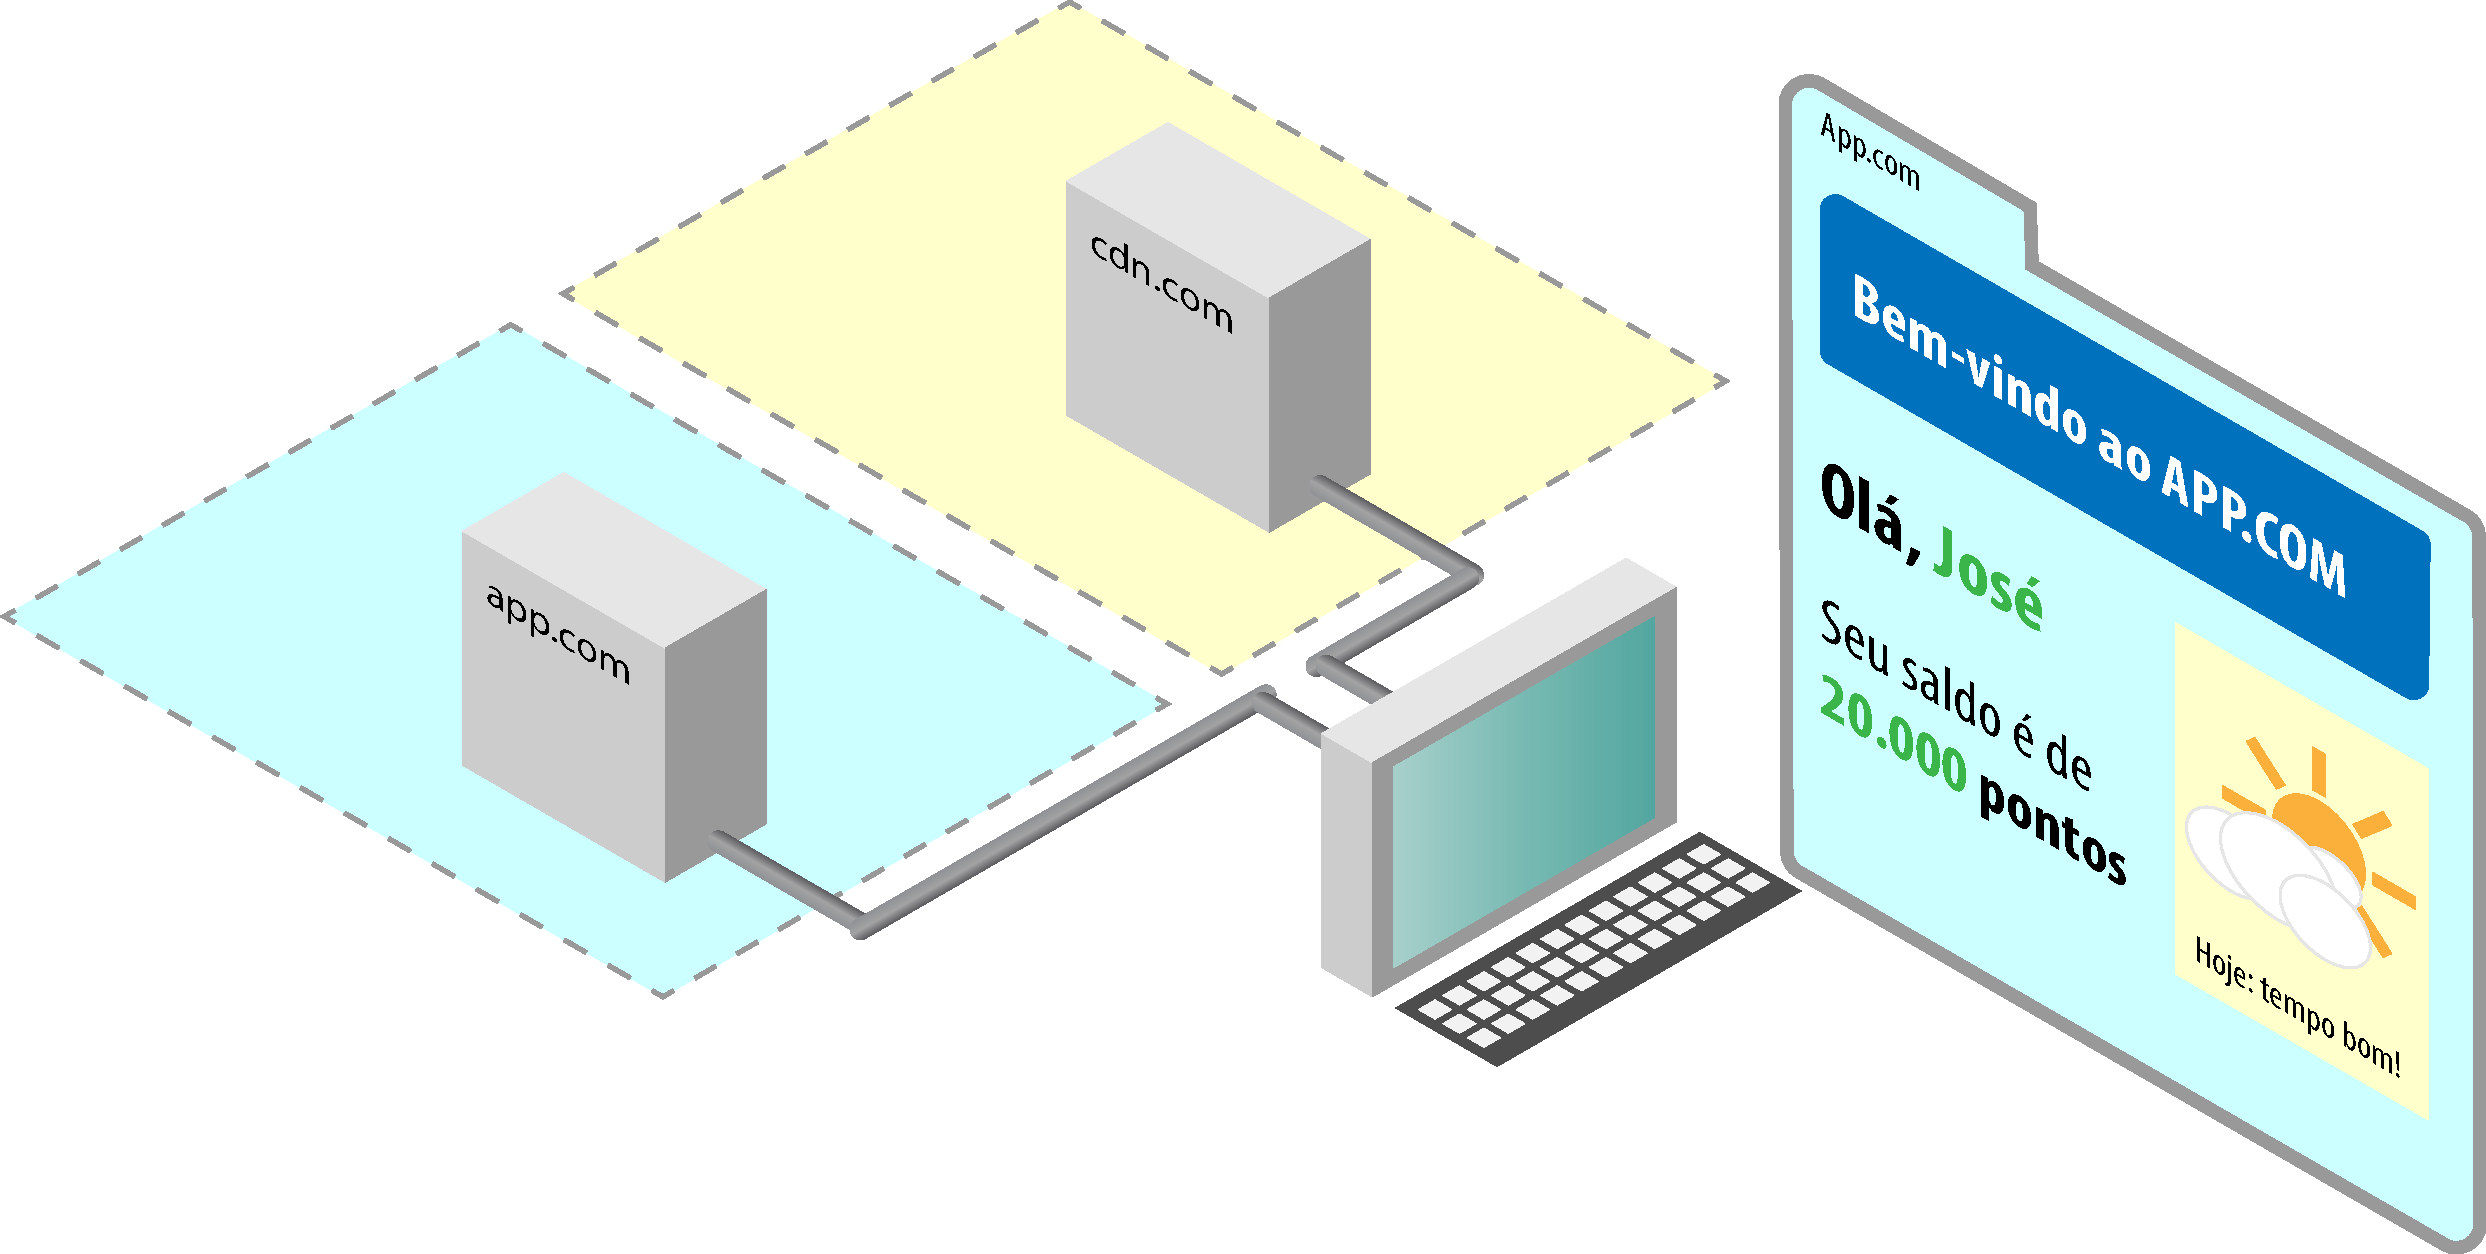
\includegraphics[width=10cm]{diagramas/diagrama01.pdf}
	\caption{Aplicação web composta por conteúdo proveniente de duas origens.}
	\label{Fig: diagrama01}
	
	\lstinputlisting[language=html,
	inputencoding=utf8,
	label={Src: webPageMultiOrigin},
	caption={[Página HTML incorporando \script de outra origem]Incorporação de \script de outra origem (linha \ref{lstCdnScript})}]{codigo/sample01-leaking-script.html}
\end{figure}

Em momento posterior, o \script servido pelos servidores da CDN é substituído por código malicioso que, além de efetuar as funções do \script benigno, captura o conteúdo da página armazenado no DOM \ref{Fig: diagrama02}. O \script pode buscar informações específicas e potencialmente sensíveis como identificação do usuário, senhas e endereços. Por causa da autorização concedida pelo protocolo CORS, o código mal intencionado tem a chance de transmitir o conteúdo capturado para um serviço anômalo.

\begin{figure}
	\centering
	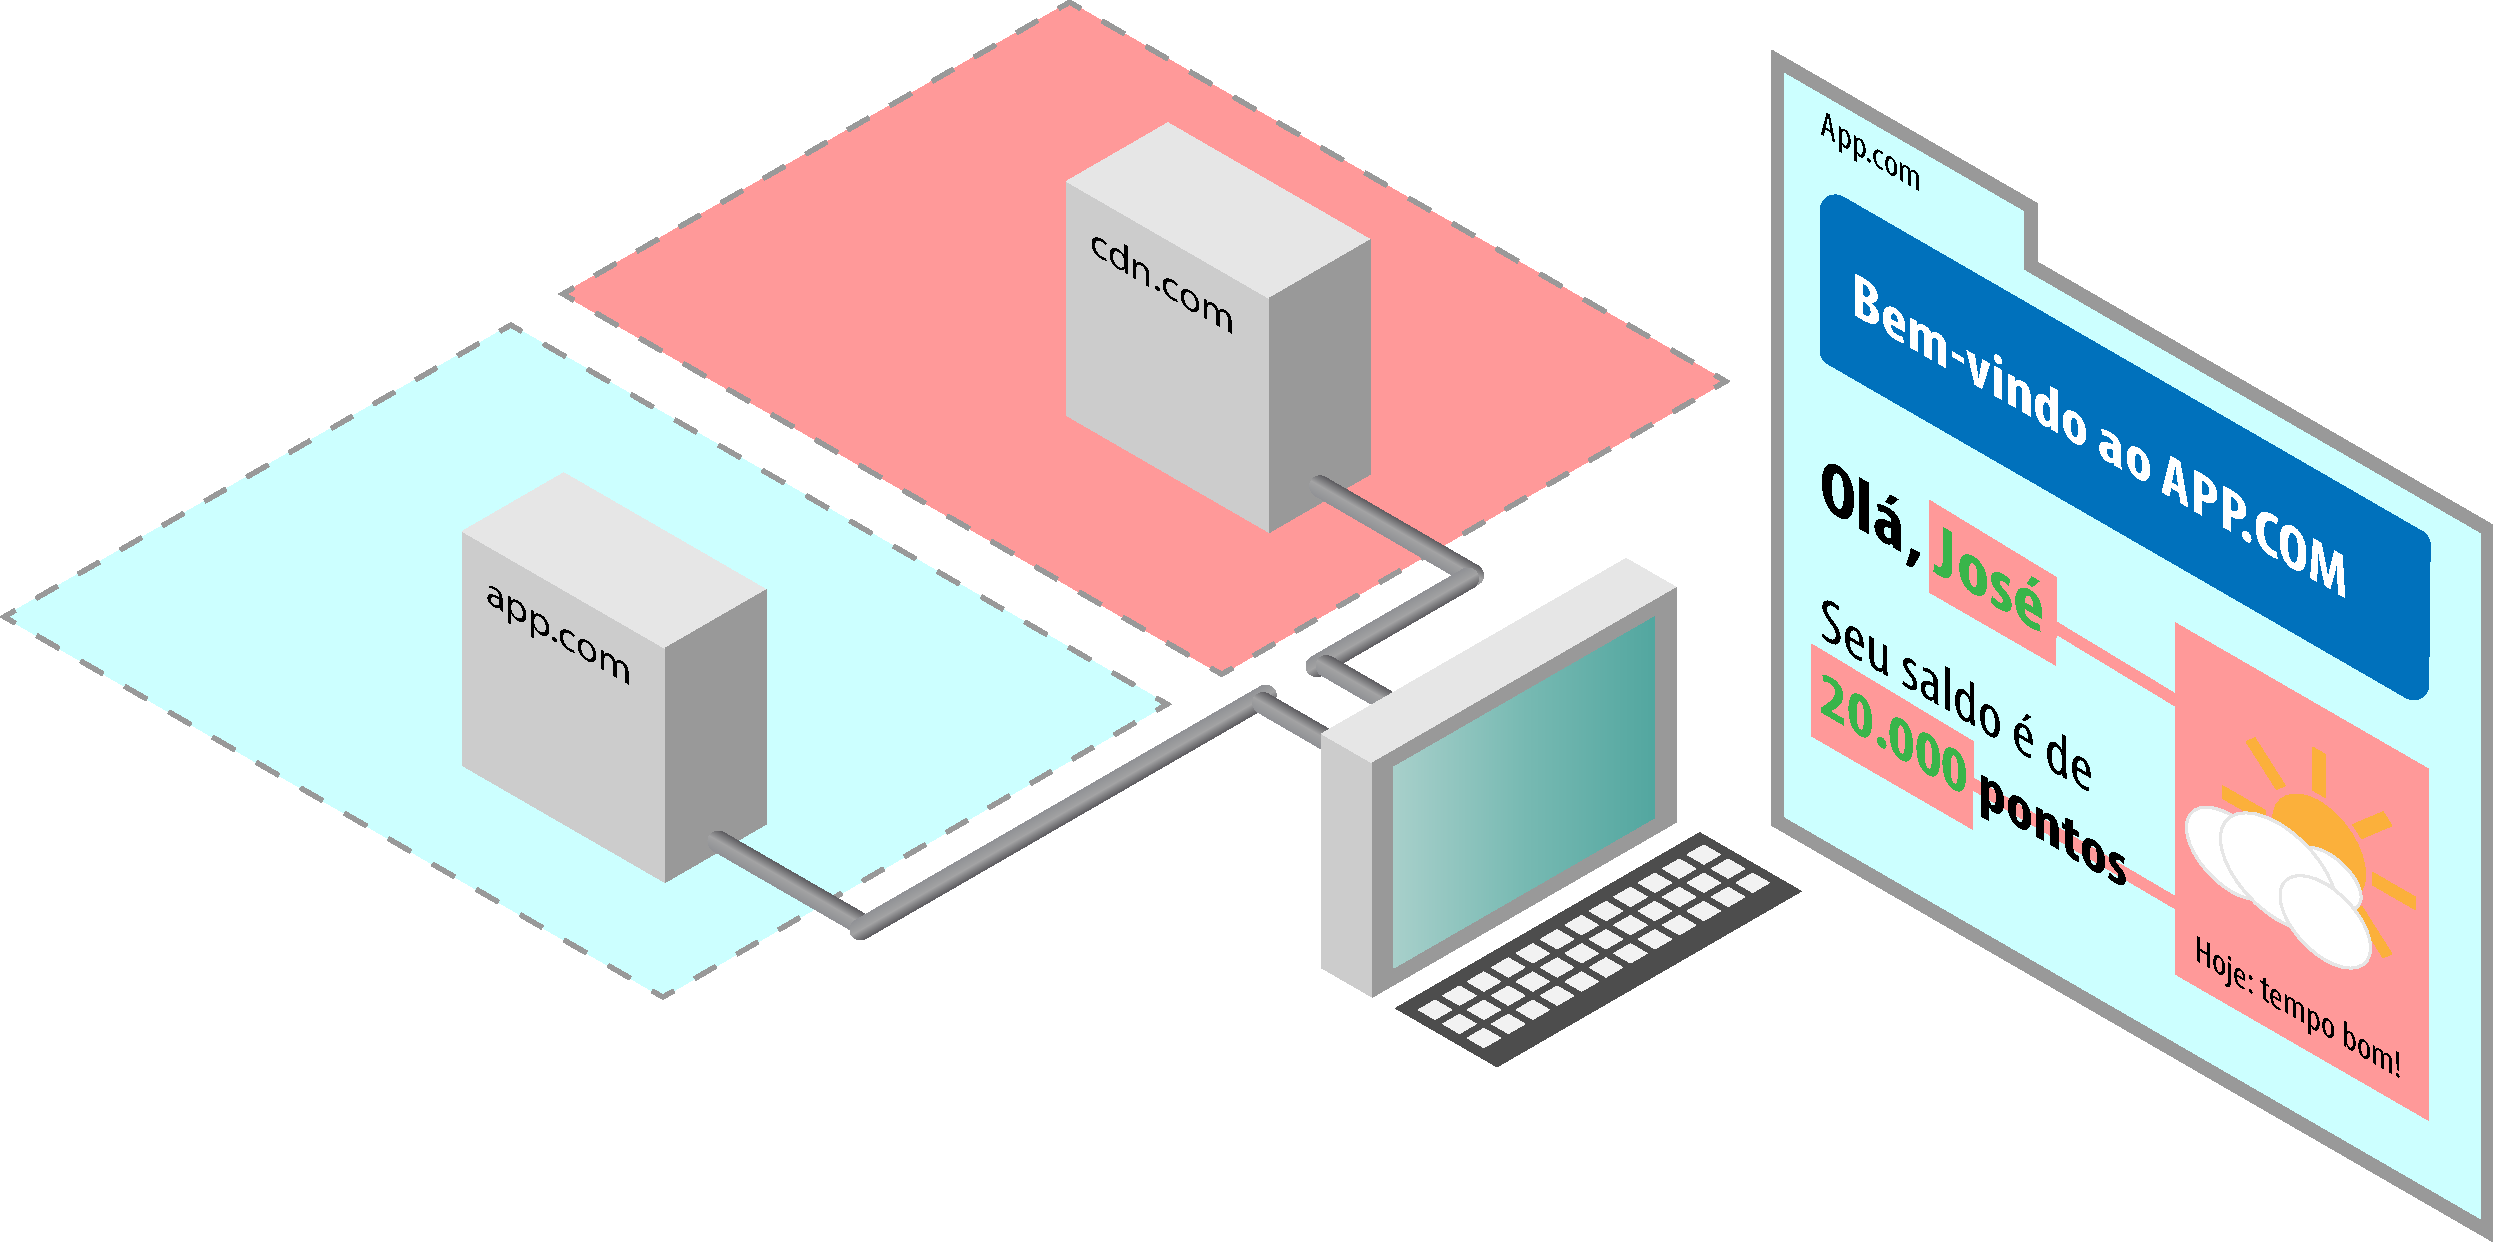
\includegraphics[width=10cm]{diagramas/diagrama02.pdf}
	\caption{Domínio de CDN comprometido, capturando informações do usuário.}
	\label{Fig: diagrama02}
\end{figure}

Acessar, capturar e modificar informações contidas no DOM também são efeitos de extensões do navegador. Mas, diferentemente dos \scripts incorporados em páginas, extensões são executadas em modo privilegiado e podem afetar todas as páginas carregadas pelo navegador, não sendo confinadas a domínios específicos. Extensões como as do Google Chrome são publicadas exclusivamente em site específico e protegido, mas não é impossível que o código fonte de extensões seja descaracterizado e publicado pela ação de \textit{hackers} \cite{Spring2017}, afetando a todos os usuários que atualizarem a extensão -- um processo automático por padrão \cite{Google2017}.


\subsubsection{Cross-Site Scripting (XSS)}
Em Javascript, todos os recursos de código carregados dentro de uma mesma página possuem os mesmos privilégios de execução. Ataques do tipo \textit{cross-site scripting} tiram proveito dessa característica para injetar código malicioso em contextos onde seja possível observar e retransmitir informação sigilosa como \textit{cookies} do usuário, endereço do navegador, conteúdo de formulários, ou qualquer outra informação mantida pelo DOM.

O emprego de medidas para prevenção de ataques XSS \cite{OWASP:XSS-CheatSheet} não elimina riscos inerentes à tecnologia do navegador. Uma vez que componentes incorporados, como anúncios e \textit{players} de mídia, conseguem carregar \scripts tidos como confiáveis dinamicamente, um único trecho de código comprometido pode colocar informações em risco sem qualquer interferência dos dispositivos de segurança.

%\subsubsection{Sobrescrita do DOM} DOM CLOBBERING

\subsubsection{Comprometimento de extensões}
Os mecanismos de extensibilidade oferecidos pelos navegadores melhoram a funcionalidade da web para os usuários, e o código de que são feitos é executado com privilégios mais elevados do que o dos \scripts incorporados pelos \textit{sites}. Por isso, os usuários precisam confirmar ao navegador que aceitam que uma extensão seja instalada, sendo informados a respeito dos privilégios que a extensão pretende utilizar. O fato de que esse processo precisa se repetir a cada vez que uma extensão necessita de um conjunto de privilégios diferente faz com que os desenvolvedores optem por solicitar, de antemão, uma gama de privilégios maior que a estritamente necessária \cite{Heule2015_Most_Dangerous_Code}.

Uma extensão que tiver sido comprometida (por exemplo, ao usar \scripts de terceiros que, por sua vez, tenham sido redirecionados ou adulterados) terá assim poder para ler e transmitir todo o conteúdo carregado e exibido pelo navegador, com o potencial de causar os mesmos efeitos observados em um ataque XSS, mas em escopo e poder aumentados, já que poderiam afetar todas as páginas abertas e todas as APIs publicadas pelo navegador.


%!TEX root = Projeto.tex

%VALE A PENA OLHAR O QUE PODE SER APROVEITADO DOS TRABALHOS ENUMERADOS COMO "SANDBOXING" NO ARTIGO SOBRE COWL.

\section{Estado da arte}
Segurança da informação é o processo de ``preservação da confidencialidade, integridade e disponibilidade da informação'' \cite{ISO2016}. Neste trabalho, tal definição será restrita aos sistemas de informação relacionados com a navegação de usuários através da web: provedores de serviço (\textit{sites}, servidores da web), protocolos de comunicação em rede (HTTP, HTTPS, \textit{web sockets}), navegadores (\textit{browsers}) e os ambientes de execução de Javascript embutidos nos navegadores. Isto delimita a área de conhecimento relevante para este trabalho.

Os objetos de estudo são (a) as vulnerabilidades derivadas dos fluxos \cite{Goguen1982} \cite{Denning1976} entre os sistemas de informação envolvidos e (b) os meios para a mitigação das vulnerabilidades. Neste capítulo será avaliado o estado da arte dos objeto de estudo fazendo, no caso de (b), uma distinção entre as abordagens ``tradicionais'' e ``experimentais'': as primeiras representam padrões já adotados na indústria e implementados nas plataformas de navegação mais comuns, enquanto as segundas incluem ferramentas e abordagens desenvolvidas experimentalmente para a solução de vulnerabilidades que, embora fundamentais, ainda não foram remediadas nativamente pelos navegadores.

%é uma preocupação desde o início da exploração comercial da web: o protocolo HTTPS, por exemplo, foi suportado pela primeira vez em 1994 pelo navegador Netscape. Mas é a partir de 1996, com a introdução da linguagem Javascript e de APIs para programação nos navegadores, que as vulnerabilidades de segurança da informação no \textit{front-end} ganharam relevância. A existência de \textit{conteúdo ativo} no navegador inaugurou um legado de preocupações sobre a confiabilidade, as finalidades e os privilégios de execução de scripts, e também dos mecanismos de segurança que ao longo do tempo foram incorporados pela indústria.

\subsection{Vulnerabilidades}

Violações de privacidade são possíveis nos navegadores por causa da natureza extremamente dinâmica da linguagem Javascript e de sua ausência de restrições de segurança em tempo de execução \cite{Jang2010}. Seus usuários estão expostos a ataques sutis com objetivos diversos como roubar \textit{cookies} e \textit{tokens} de autorização, redirecionar o navegador para sites falsos (\textit{phishing}), observar o histórico de navegação e rastrear o comportamento do usuário através dos movimentos do ponteiro do mouse e eventos de teclado. Para que scripts mal-intencionados sejam incorporados a páginas benignas, \textit{hackers} fazem uso de vulnerabilidades como \textit{cross-site scripting (XSS)} \cite{OWASP:XSS} e comprometimento de extensões \cite{Heule2015}, problemas para os quais os navegadores não oferecem ainda proteção total.

\subsubsection{Cross-Site Scripting (XSS)}
Em Javascript, todos os recursos de código carregados dentro de uma mesma página possuem os mesmos privilégios de execução. Ataques do tipo \textit{cross-site scripting} tiram proveito dessa característica para injetar código malicioso em contextos onde seja possível observar e retransmitir informação sigilosa como \textit{cookies} do usuário, endereço do navegador, conteúdo de formulários, ou qualquer outra informação mantida pelo DOM.

O emprego de medidas para prevenção de ataques XSS \cite{OWASP:XSS-CheatSheet} não elimina riscos inerentes à tecnologia do navegador. Uma vez que componentes incorporados, como anúncios e \textit{players} de mídia, conseguem carregar scripts tidos como confiáveis dinamicamente, um único trecho de código comprometido pode colocar informações em risco sem qualquer interferência dos dispositivos de segurança.

\subsubsection{Comprometimento de extensões}

Os mecanismos de extensibilidade oferecidos pelos navegadores\footnote{``Extensões'' e \textit{``apps''} do Chrome; e ``complementos'' do Firefox e do Internet Explorer} melhoram a funcionalidade da web para os usuários, e o código de que são feitos é executado com privilégios mais elevados do que o dos scripts incorporados pelos \textit{sites}. Por isso, os usuários precisam confirmar ao navegador que aceitam que uma extensão seja instalada, sendo informados a respeito dos privilégios que a extensão pretende utilizar. O fato de que esse processo precisa se repetir a cada vez que uma extensão necessita de um conjunto de privilégios diferente faz com que os desenvolvedores optem por solicitar, de antemão, uma gama de privilégios maior que a estritamente necessária \cite{Heule2015}.

Uma extensão que tiver sido comprometida (por exemplo, ao usar scripts de terceiros que, por sua vez, tenham sido redirecionados ou adulterados) terá assim poder para ler e transmitir todo o conteúdo carregado e exibido pelo navegador, com o potencial de causar os mesmos efeitos observados em um ataque XSS, mas em escopo e poder aumentados, já que poderiam afetar todas as páginas abertas e todas as APIs publicadas pelo navegador.

\subsection{Abordagens tradicionais para contenção de ataques}

\subsubsection{SOP -- Same Origin Policy}
Implementada desde o primeiro navegador com suporte a Javascript, SOP \cite{W3C:SOP} é uma política que impõe limites aos meios pelos quais uma página ou script efetuam requisições a recursos que se encontram em \textit{domínios diferentes}\footnote{``Domínios'' identificam origens de recursos pela combinação do protocolo, do nome do host e da porta utilizados para o acesso ao recurso.}. SOP promove isolamento de informações ao impedir que o conteúdo em um domínio acesse conteúdo que tenha sido carregado em domínios diferentes.

Na prática, essa política restringe funcionalidades importantes sem solucionar completamente o problema do vazamento de informações. SOP impede, por exemplo, que um script inicie requisições assíncronas\footnote{Através das	APIs Ajax e XHR} para outros domínios, ao mesmo tempo em que permite que um script incorporado através de XSS efetue vazamento da identidade do usuário. Em geral, os navegadores diminuem certas restrições da SOP para permitir APIs mais funcionais, e implementam meios mais flexíveis para proteção contra ataques de XSS.

\subsubsection{CSP -- Content Security Policy}
CSP foi criada como um complemento à SOP, elevando a capacidade do navegador de servir como plataforma razoavelmente segura para composição de aplicações \textit{mashup} ao estabelecer um protocolo para o compartilhamento de dados entre os componentes da página que residam em domínios diferentes. CSP define um conjunto de diretivas (codificadas como cabeçalhos HTTP) para a definição de \textit{whitelists} -- o conjunto de origens confiáveis em um dado momento -- pelas quais navegador e provedores de conteúdo estabelecem o controle de acesso e o uso permitido de recursos embutidos como scripts, folhas de estilos, imagens e vídeos, entre outros. Através desse protocolo, ataques de XSS que podem ser neutralizados desde que todos os componentes na página sejam aderentes à mesma política de CSP.

\subsubsection{CORS -- Cross-Origin Resource Sharing}
Assim como a CSP, o mecanismo CORS \cite{W3C:CORS} complementa a SOP estabelecendo um conjunto de diretivas (cabeçalhos HTTP) para a negociação de acesso via Ajax/XHR a recursos hospedados em domínios diferentes. CORS determina que exista um vínculo de confiança entre navegadores e provedores de conteúdo, dificultando vazamento de informação ao mesmo tempo em que flexibiliza as funcionalidades das APIs. O uso de CORS permite que os autores de componentes e desenvolvedores de aplicações \textit{mashup} determinem o grau de exposição que cada conteúdo pode ter em relação aos outros conteúdos incorporados.

CSP e CORS são recomendações do comitê W3C \cite{W3C:CSP} \cite{W3C:CORS}, sendo incorporados por todos os navegadores relevantes desde 2016 \cite{CanIUse:CSP} \cite{CanIUse:CORS}.


\subsection{Abordagens experimentais para contenção de ataques}
Os mecanismos tradicionais são discricionários, pois as aplicações devem pré-estabelecer explicitamente seus parâmetros de segurança da informação (seja através de CSP ou CORS) para que o navegador configure um contexto de segurança correspondente \cite[p. 31]{stefan:2015:phdthesis}. Trata-se, ademais, de um controle estático, imutável durante todo o ciclo de vida da página, o que é inadequado para aplicações ao estilo \textit{mashup} em que os componentes da página podem ser desconhecidos no momento em que as diretivas de segurança são aplicadas pelo navegador.

Uma característica fundamental das abordagens tradicionais é sua ênfase na comunicação de rede entre domínios distintos. Esse é um enfoque pertinente: a confiabilidade entre domínios é essencial para garantir um mínimo de segurança. No entanto, o navegador como um todo pode abrir vulnerabilidades que independem de conexões de rede para se concretizarem. \textit{Plugins} e extensões são executados com privilégios elevados e têm acesso a todas as partes do navegador com as quais os usuários interagem, podendo extender dinamicamente a linguagem Javascript para modificar seu funcionamento e rastrear de informações.

Abordando a segurança da informação no navegador de forma holística, mecanismos experimentais têm sido propostos para implementar \textit{controle do fluxo de informação} (IFC -- \textit{information flow control}) como estratégia de segurança não-discricionária e dinâmica.


\subsubsection{An empirical study of privacy-violating information flows in JavaScript web applications \cite{Jang2010}}
Este artigo é um dos primeiros trabalhos relevantes sobre as vulnerabilidades expostas pela linguagem JavaScript e seu tratamento através de IFC. Os autores apresentam situações em que scripts maliciosos podem subverter o comportamento normal das aplicações e causar falhas de segurança da informação. É proposto um mecanismo de detecção e neutralização desse tipo de ataque.

\textbf{Contribuição.} A formalização das vulnerabilidades na linguagem JavaScript, a metodologia dos testes efetuados e a natureza da ferramenta descrita no artigo serviram como referenciais para a proposição de novas abordagens, algumas das quais são referenciadas nesta pesquisa. De forma presciente, os autores apontam o IFC como um caminho a ser seguido. Diversas iniciativas posteriores, algumas revisadas neste documento, seguem nessa direção.


\subsubsection{Security of web mashups: A survey \cite{DeRyck2012}}
O artigo é motivado pelos requisitos de segurança de aplicações \textit{mashup}. Os autores definem um conjunto de categorias de requisitos não funcionais de segurança e avaliam a conformidade desses requisitos versus funcionalidades do navegador. O critério de classificação estabelecido posiciona as diversas abordagens em quatro graduações que vão desde a separação total de componentes até sua integração completa.

\textbf{Contribuição.} O artigo contribui com a enumeração de requisitos que uma solução voltada à segurança da informação deve atender. Algumas das tecnologias mencionadas podem ter se tornado obsoletas ou de alcance limitado desde que o artigo foi escrito, o que não invalida o resultado pretendido pelos autores, que é considerado ``estado da arte'' \cite{Hedin2014} em pesquisa sobre segurança de aplicações de composição baseadas em Javascript.


\subsubsection{Information-Flow Security for a Core of JavaScript \cite{Hedin2012}}
Este trabalho contém uma proposta conceitual para mitigação dos problemas de segurança da informação inerentes à implementação e execução da linguagem Javascript nos navegadores modernos. Apresentando casos de uso comuns, os autores empregam o conceito de \textit{não-interferência} para introduzir um monitor de execução como sentinela de uso indevido de informação no sistema dinâmico de tipos em Javascript. O trabalho, puramente conceitual, alcança esse objetivo através da extensão de um subconjunto fundamental \textit{(core)} da linguagem que, partindo da definição formal de Javascript\footnote{ECMA-262 -- \url{http://www.ecma-international.org/publications/standards/Ecma-262.htm}}, introduz anotações de código fonte que permitem a composição de programas à prova de vazamento de informação.

\textbf{Contribuição.} Este trabalho fornece uma prova da eficácia das abordagens baseadas no controle do fluxo de informações (IFC). Por se tratar de um exercício teórico, e propositalmente limitado a um subconjunto da linguagem, o conteúdo serve como introdução aos desafios e conceitos associados ao IFC. Por fim, a simplicidade e o rigor da solução apresentada também funcionam como exemplos a serem seguidos.


\subsubsection{Toward Principled Browser Security \cite{Yang2013}}
Os autores analisam criticamente os mecanismos tradicionais SOP, CORS e CSP para expor suas heurísticas e políticas \textit{ad-hoc} que, em troca de flexibilidade, abrem diversas vulnerabilidades de segurança da informação. Partindo dessa condição, e motivados pela robustez das abordagens de controle do fluxo de informações, os autores propõem um modelo baseado em IFC que, mesmo suportando todas as heurísticas existentes, é resistente aos algoritmos de ataque.

\textbf{Contribuição.} Este artigo enriquece o repertório a respeito de IFC aplicando essa abordagem ao escopo das funcionalidades além da execução de Javascript.


\subsubsection{JSFlow: Tracking information flow in JavaScript and its APIs \cite{Hedin2014}}
O trabalho, uma continuação de outro de mesma autoria\cite{Hedin2012}, é composto de duas partes: primeiro, os autores descrevem o panorama geral das pesquisas em segurança da informação em Javascript, detalhando as vulnerabilidades mais comuns e propondo como solução o controle do fluxo de informações; e em segundo, apresentam o projeto JSFlow\footnote{JSFlow -- \url{http://www.jsflow.net/}}, uma implementação da linguagem Javascript com IFC puramente dinâmico integrado. Disponibilizado tanto através de extensão de navegador como ainda módulo \textit{back-end} para o ambiente Node.js, e escrito na própria linguagem Javascript, JSFlow oferece segurança da informação de forma transparente e ubíqua, abrangendo a totalidade dos scripts executados no navegador -- ainda que de modo experimental. O trabalho é concluído com um teste da eficácia do software.

\textbf{Contribuição.} O escopo do projeto JSFlow demonstra até que ponto é possível adotar uma abordagem puramente dinâmica para IFC. Fica evidente que tal abordagem abre oportunidade para a existência de ``falsos positivos'' durante a avaliação dos níveis de segurança associados a cada contexto de execução, um problema que os autores propõem mitigar através de uma abordagem estática complementar (ao que denominam ``análise híbrida''). Outros trabalhos, ainda fora do escopo desta presente pesquisa, exploram essa alternativa.


\subsubsection{Information Flow Control in WebKit's JavaScript Bytecode \cite{Bichhawat2014}}
Levando a análise do fluxo de informações a um patamar ainda mais profundo, este trabalho introduz um monitor de segurança integrado ao compilador de Javascript do mecanismo WebKit de navegação\footnote{O projeto de código aberto WebKit serve como base para a construção de navegadores como o Safari (MacOS e iOS).}. Os autores discorrem sobre os desafios de se implementar um monitor dinâmico operando sobre o \textit{bytecode} gerado pelo compilador, enfatizando a dificuldade de tratamento de fluxos não-estruturados, porém válidos, na linguagem Javascript -- especificamente, programas que fazem uso de instruções como \texttt{break}, \texttt{throw}, \texttt{continue}, \texttt{return} etc. Os autores demonstram como a análise estática é mais apropriada que a análise dinâmica para a avaliação de \textit{bytecode}. Preocupações com o desempenho do monitor e seu \textit{overhead} comparado às implementações padrão do WebKit são endereçadas com uma bateria de testes realizada através da suíte SunSpider\footnote{SunSpider -- \url{https://webkit.org/perf/sunspider/sunspider.html} (descontinuado; sucedido pela suíte JetStream, disponível em \url{http://browserbench.org/JetStream/})}.

\textbf{Contribuição.} O trabalho deixa evidente a complexidade e o esforço necessário para a implementação de um projeto dessa envergadura. Desconsiderando a natureza prototípica do artefato de software derivado do trabalho, os autores expõem com clareza o funcionamento do \textit{bytecode} gerado a partir de Javascript sob o ponto de vista da segurança da informação, apontando, como \cite{Hedin2014}, para a análise híbrida como o meio mais adequado para a avaliação de níveis de segurança em fluxos não-estruturados.


\subsubsection{Protecting Users by Confining JavaScript with COWL \cite{Stefan2014}}
O artigo argumenta que, face às dificuldades que os desenvolvedores encontram para aderir aos mecanismos tradicionais SOP, CSP e CORS, acaba-se optando pela funcionalidade em detrimento da segurança. Isto se manifesta em extensões de navegador solicitando mais permissões do que o necessário, em \textit{mashups} que requerem autorizações desnecessárias para o usuário, e em notificações de segurança tão constantes que se tornam efetivamente invisíveis. Entendendo que o estado-da-arte da análise do fluxo de informações em navegador é deficiente -- seja porque as ferramentas são incompletas ou porque degradam desempenho --, os autores apresentam o projeto COWL\footnote{COWL: Confinement with Origin Web Labels -- \url{http://cowl.ws/}}, implementanto o conceito de ``controle de acesso mandatório''\footnote{Tradução livre para o termo \textit{mandatory access control}.}onde os desenvolvedores definem quais informações são restritas e quem são os atores que podem acessar essas informações, relegando ao COWL o monitoramento da política de segurança. A esse estilo de IFC os autores denominam ``granularidade ampla''\footnote{Idem para o termo \textit{coarse-grained}.} uma vez que a política de segurança se aplica a contextos de execução inteiros, em contraste com a ``granularidade fina''\footnote{Idem para o termo \textit{fine-grained}.} em que a aplicação da política recai sobre objetos específicos.

\textbf{Contribuição.} A separação das iniciativas de IFC por níveis de granularidade efetivamente recontextualiza o conceito de controle de fluxo de informação. Além disso, a iniciativa COWL é um projeto em andamento, documentado e em vias de se tornar uma API padrão pelo W3C\footnote{\url{https://w3c.github.io/webappsec-cowl/}}.


\subsubsection{Architectures for inlining security monitors in web applications \cite{Magazinius2014}}
Este trabalho avalia diferentes arquiteturas que podem ser aplicadas para efetuar checagem de segurança \textit{inline} (incorporado ao código fonte previamente sua execução). Os autores listam quatro arquiteturas -- extensões de navegador, proxies HTTP, proxies por prefixo e através de integradores.
O artigo explora prós e contras de cada uma, considerando as garantias de segurança envolvidas. O trabalho é complementado pela implementação experimental das arquiteturas, empregando como monitor o JSFlow \cite{Hedin2014}.

\textbf{Contribuição.} O artigo é inovador ao propor uma diversidade de arquiteturas e, consequentemente, de \textit{stakeholders} para controle de fluxo de informações. Partindo disso, os autores concluem que existem diversas oportunidades para avanço e funcionalidades ainda vulneráveis a ataques por não se enquadrarem no foco das pesquisas nesta área, como scripts de origens heterodoxas (fora de elementos \texttt{<sctipt>}).


\subsubsection{Information Flow Control for Event Handling and the DOM in Web Browsers \cite{Rajani2015}}
\textbf{Resumo.} O trabalho explora vulnerabilidades no fluxo de informações em scripts acionados por eventos do navegador (tecnicamente, eventos do DOM). Tais vulnerabilidades são inerentes ao modo como os navegadores executam eventos e como isso se reflete, negativamente, nos monitores de IFC. Os autores partem da abordagem híbrida descrita em \cite{Bichhawat2014} para criar um monitor à prova de vazamento de informação, com baixo \textit{overhead}, e o colocam em comparação com iniciativas como \cite{Stefan2014} e \cite{Hedin2014}.


	%!TeX spellcheck = pt_BR
%!TEX root = Projeto.tex
\chapter{Proposta (Em desenvolvimento)}

%!TeX spellcheck = pt_BR
%!TEX root = Projeto.tex

\section{API de ocultação do DOM fundamentada em Shadow DOM}
\tbc
%!TeX spellcheck = pt_BR
%!TEX root = Projeto.tex

\section{Casos de teste de exposição aos riscos de vazamento de informação no navegador}
\tbc
%!TeX spellcheck = pt_BR
%!TEX root = Projeto.tex

\section{Apresentação do site acadêmico ``jstest.me''}
\tbc

\section{Roteiro para a elaboração da proposta}

\begin{alineas}
	\item \textbf{Mapeamento de cenários.} Partindo dos requisitos não funcionais estabelecidos, serão definidos cenários de testes capazes de evidenciar as condições necessárias para a não-conformidade com esses requisitos. Os cenários assim definidos delimitarão o escopo de ação da abordagem proposta por este trabalho.
	\item \textbf{Especificação da proposta.} A abordagem derivada dos cenários de testes será formalmente especificada, em termos das interfaces e funcionalidades esperadas, visando orientar o desenvolvimento de uma implementação de teste e provas de conceito.
	\item \textbf{Implementação do mecanismo de ocultação.} A materialização da abordagem proposta será efetuada pelo desenvolvimento dos scripts necessários para a implementação das interfaces esperadas, em conformidade com os requisitos funcionais esperados.
	\item \textbf{Validação.} Os cenários de testes serão implementados na forma de provas de conceito para validação da proposta e do mecanismo implementado. O objetivo é conhecer a aderência do mecanismo em relação aos requisitos.
\end{alineas}
	
	% ----------------------------------------------------------
	% ELEMENTOS PÓS-TEXTUAIS
	% ----------------------------------------------------------
	\postextual
	%!TEX root = Projeto.tex
% ----------------------------------------------------------
% Referências bibliográficas
% ----------------------------------------------------------
\setboolean{isBib}{true} % Obriga o titulo das referências à esquerda

\setlength\bibitemsep{12pt} % Espaço de uma linha entre as referencias

\bibliography{Projeto}

\setboolean{isBib}{false} % Desobriga o titulo das referências à esquerda

% ----------------------------------------------------------
% Apêndices
% ----------------------------------------------------------

%\apendices
%\partapendices
%\chapter{Lorem ipsum dolor sit amet}

%\lipsum[21-26]

% ----------------------------------------------------------
% Anexos
% ----------------------------------------------------------

% \anexos
% \partanexos
% \chapter{Padrões de projeto para mitigação de riscos}

\section{}
%\lipsum[26-32]

	
	
	
\end{document}
